\section{Introduction}

%%%%%%%%%%%%%%%%%%%%%%%%%%%%%%%%%%%%%%%%%%%%%%%%%%%%%%%%%%
%%%%%%%%%%%%%%%%%%%%outline%%%%%%%%%%%%%%%%%%%%%%
%%%%%%%%%%%%%%%%%%%%%%%%%%%%%%%%%%%%%%%%%%%%%%%%%%%%%%%%%%
\begin{frame}\frametitle{What goes into a BEAST model?}
  \begin{figure}
      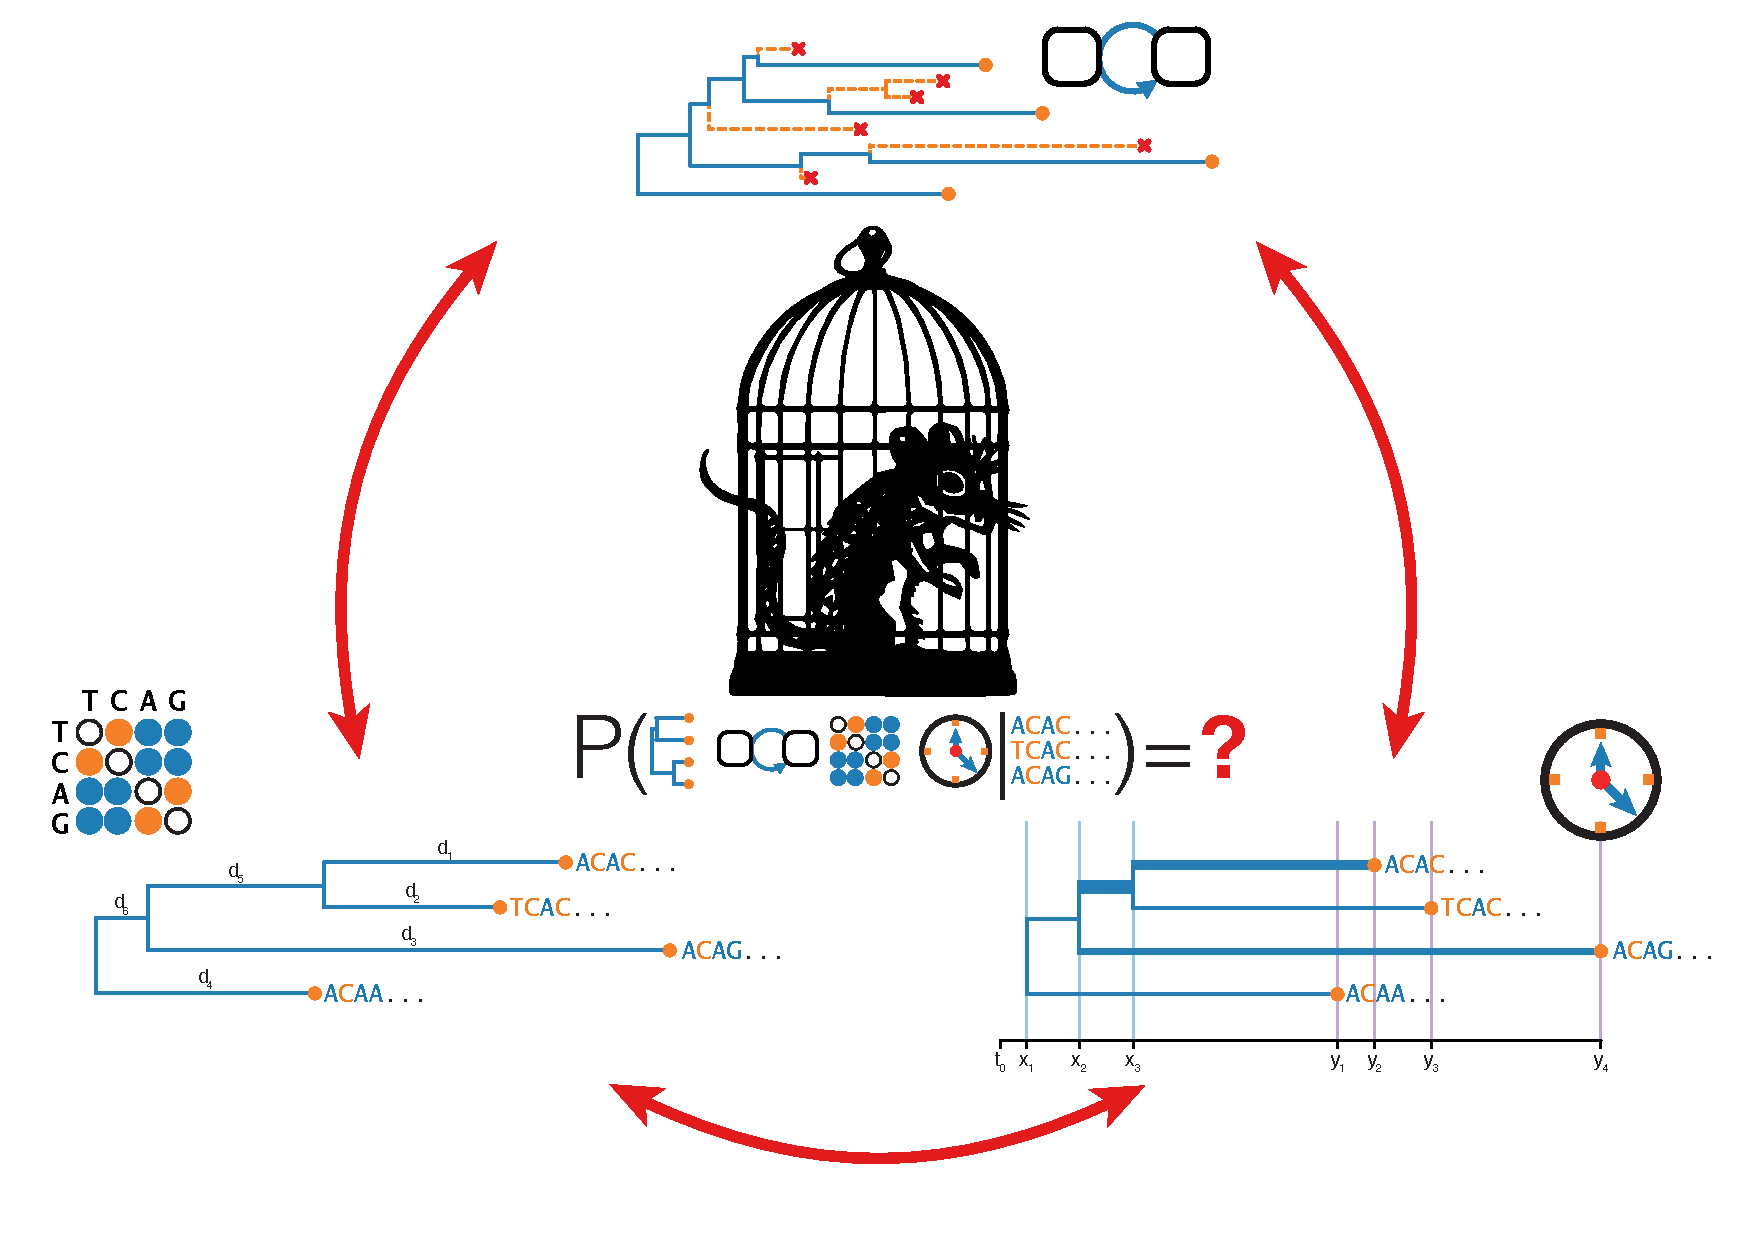
\includegraphics[width=0.9\textwidth]{figures/Taming-the-BEAST-Splash.pdf}
  \end{figure}
    \begin{figure}
      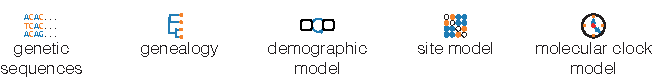
\includegraphics[width=0.9\textwidth]{figures/ModelComponents.pdf}
  \end{figure}
\end{frame}

\begin{frame}\frametitle{What is a model?}
      Model consists of:
        \begin{itemize}
            \item Tree prior
            \item Site model
            \item Clock model
            \item Priors
            \item Hyperpriors
        \end{itemize}

      \vspace{1cm}
      How can we decide which model components to use?

      \begin{itemize}
           \item \textbf{Model selection:} Which model is better?
           \item \textbf{Model adequacy:} Is the model any good?
           \item \textbf{Model averaging:} If you don't want to choose...
       \end{itemize}
      
\end{frame}

\section{Model selection}

\begin{frame}\frametitle{Bayesian phylogenetics}

  Posterior:
  \[
      p(\theta | D) = \frac{p(D | \theta) p(\theta)}{p(D)}
  \]

  \pause

  Should actually write:
  \[
      p(\theta | D, M) = \frac{p(D | M, \theta) p(\theta | M)}{p(D | M)}
  \]

  \begin{itemize}
    \item $D$: Data
    \item $M$: Model
    \item $\theta$: Particular parameterization of model $M$
  \end{itemize}

  \vspace{0.5cm}

  \pause
  $P(D | M)$ is the marginal probability of the data under model $M$

\end{frame}


\begin{frame}\frametitle{Marginal likelihood of the data}

  Need to calculate the marginal likelihood of the data to do Bayesian model selection:

  \[
      P(D | M) = \int_\theta P(D | M, \theta)P(\theta | M) d\theta
  \]

  \pause
  Calculate Bayes factors:

  \[
      BF_{M_1,M_2} = \frac{P(D | M_1)}{P(D | M_2)}
  \]

  \pause
  \vspace{0.5cm}

  \begin{itemize}
    \item Models do \textbf{not} need to be nested!
    \item Cannot compare models on \textbf{different} datasets! 
    \item $P(D | M)$ is \textbf{difficult} to calculate!
  \end{itemize}

\end{frame}


\begin{frame}\frametitle{Approximate marginal likelihood of the data}

  \textbf{In Tracer:}

    \begin{itemize}
      \item HME (Harmonic mean estimate)
      \item AIC$_M$
    \end{itemize}

    \pause
    ``The total unsuitability of the harmonic mean estimator should have been apparent within an hour of its discovery.'' - Radford Neal \scriptsize{(\url{http://radfordneal.wordpress.com/2008/08/17/the-harmonic-mean-of-the-likelihood-worst-monte-carlo-method-ever})}
    
    \normalsize
    \pause
    \vspace{0.25cm}
    Only use the AIC$_M$ if you are short on time!
    \vspace{0.5cm}
  \pause

  \textbf{In BEAST and BEAST2:}
    \begin{itemize}
      \item Stepping stone
      \item Path-sampling
    \end{itemize}

    \pause
    Stepping stone and path-sampling are the best that is currently available!
\end{frame}

\begin{frame}\frametitle{Model selection in Tracer}

  \begin{figure}
      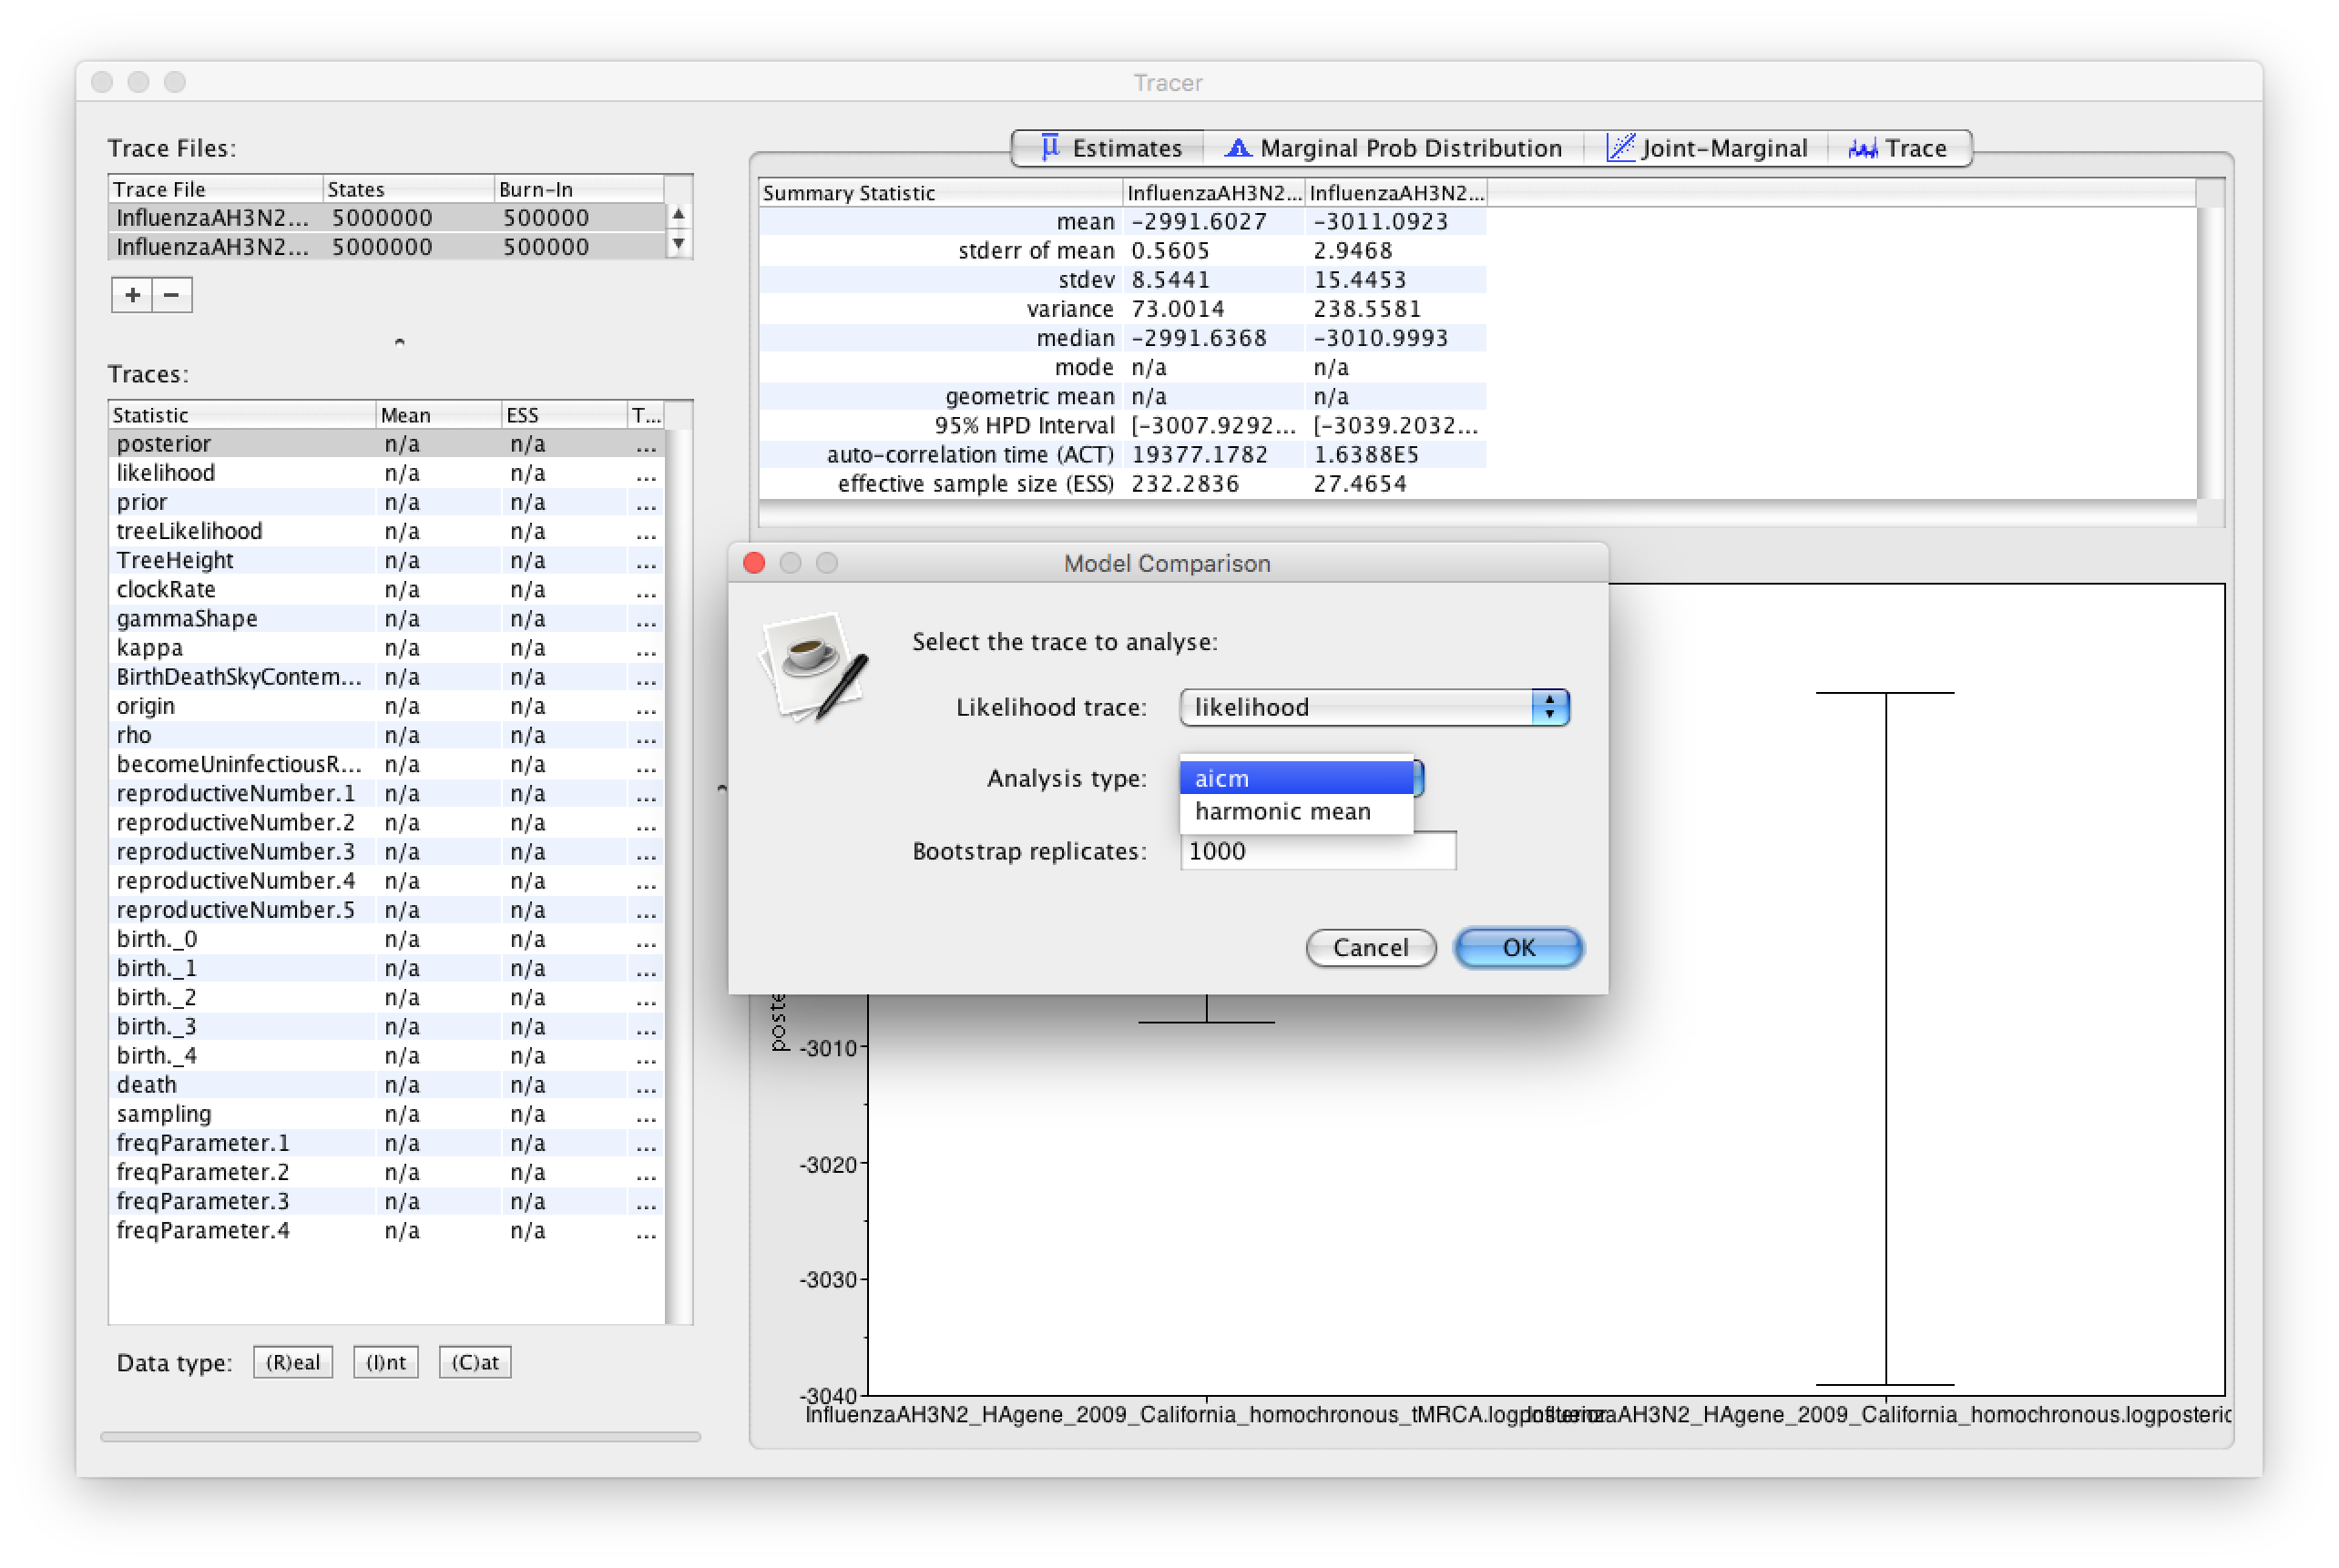
\includegraphics[width=\textwidth]{figures/TracerModelSelection}
  \end{figure}

\end{frame}

\begin{frame}\frametitle{Model selection in BEAST2}

  \begin{figure}
      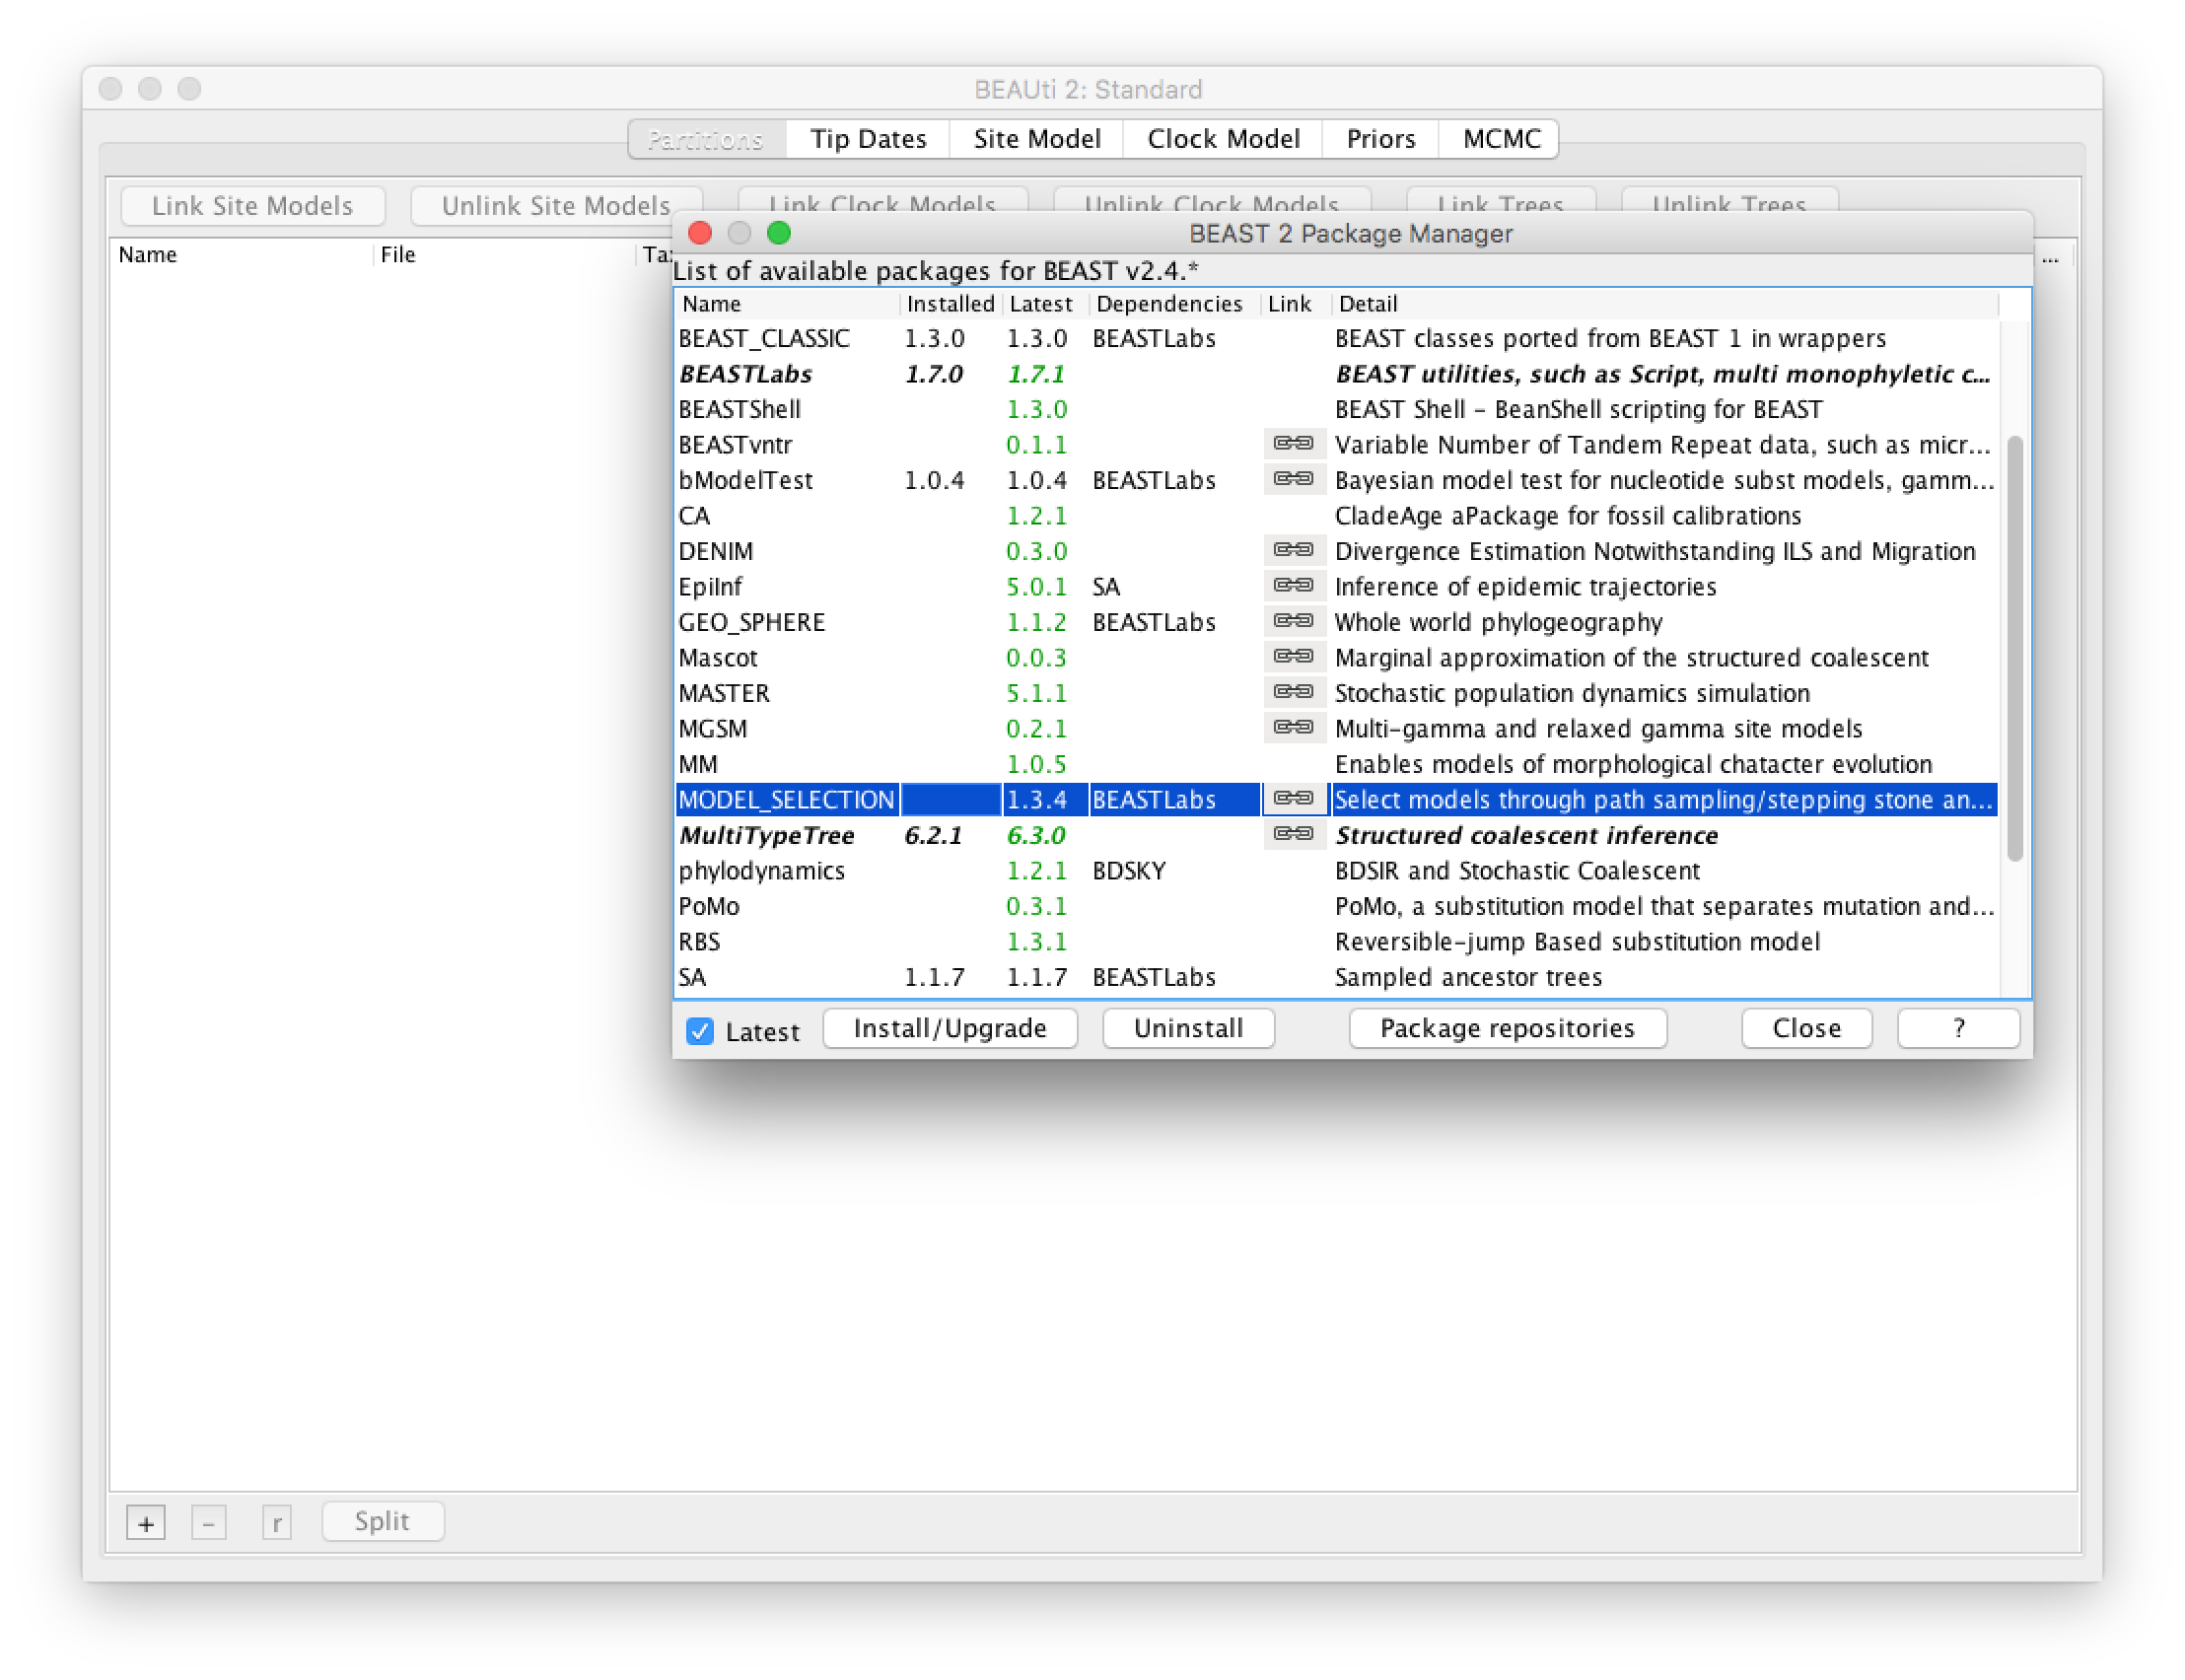
\includegraphics[width=\textwidth]{figures/BeautiModelSelection1}
  \end{figure}

\end{frame}

\begin{frame}\frametitle{Model selection in BEAST2}

  \begin{figure}
      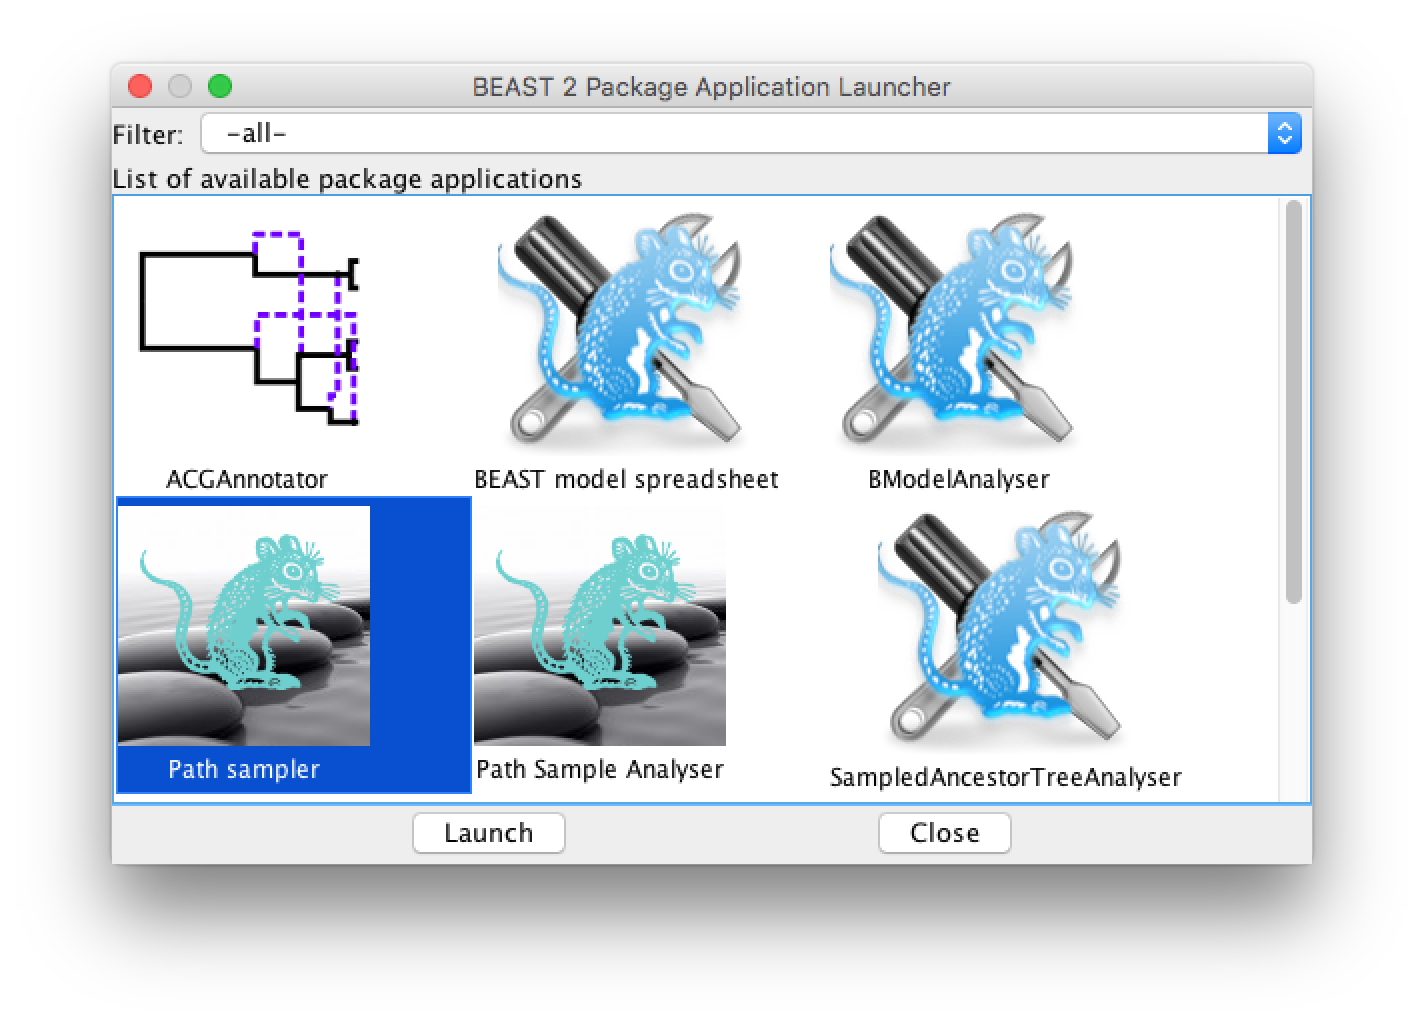
\includegraphics[width=0.5\textwidth]{figures/BeautiModelSelection2}
  \end{figure}

\end{frame}

\section{Model averaging}

\begin{frame}\frametitle{Nuisance parameters}

  Marginalization:

  \[
    P(\phi) = \int_\theta P(\phi,\theta)d\theta = \int_\theta P(\phi | \theta) P(\theta) d\theta
  \]

  \begin{itemize}
    \item We can get rid of parameters we are not interested in by integrating them out!
    \item Effectively taking an average across all possible values of the parameter
    \item Estimates remaining parameters while taking into account uncertainty in nuisance parameters
  \end{itemize}

  \pause
  e.g. BEAST naturally takes into account phylogenetic uncertainty by integrating over all possible tree topologies!

\end{frame}


\begin{frame}\frametitle{Model averaging}

  We can actually integrate out components of the model in the same way!
  (nuisance models?)

  \vspace{0.5cm}
  \textbf{Reversible-jump MCMC (RJMCMC):}

  \begin{itemize}
    \item Specify the state space of different models
    \item Need to tell your MCMC sampler how to step between different models
    \item Not easy to implement correctly (see \cite{Green1995})
  \end{itemize}
  
\end{frame}

\begin{frame}\frametitle{Simple example}

  \begin{figure}
      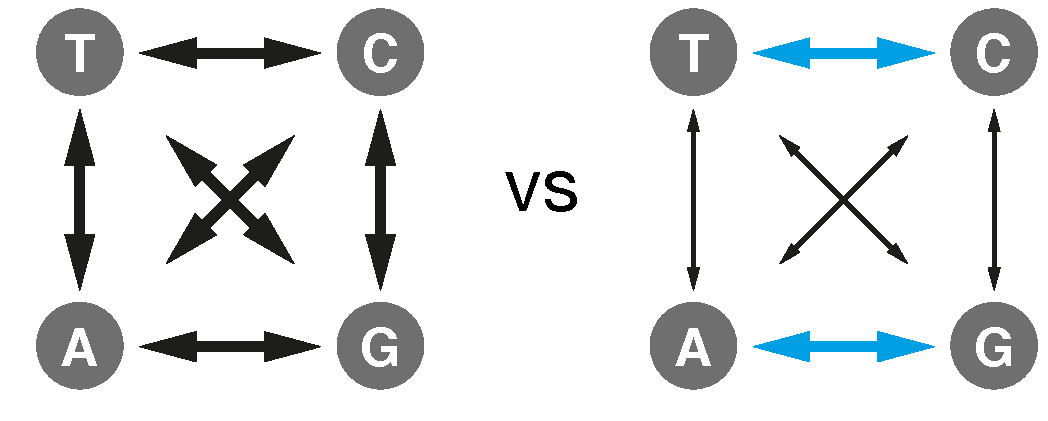
\includegraphics[width=0.8\textwidth]{figures/jc69vsk80.pdf}
  \end{figure}


  Stepping from JC69 to K80 means introducing an extra parameter

\end{frame}

\begin{frame}\frametitle{BModelTest}

  Averages over different nucleotide substitution models

  \begin{figure}
      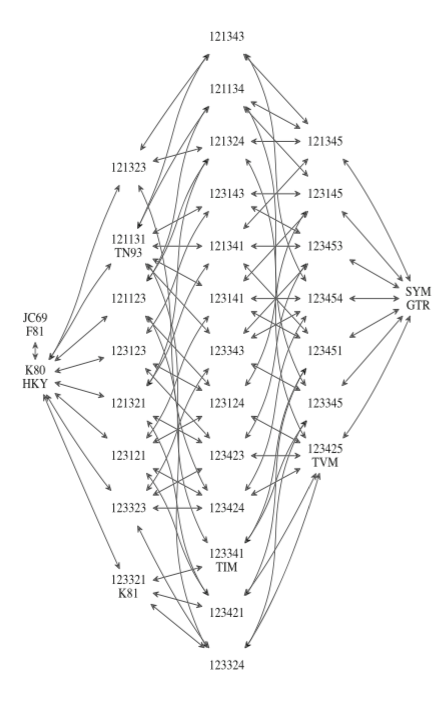
\includegraphics[height=0.7\textheight]{figures/BModelTest}
      \figureCaption{\cite{Bouckaert2017}}{All models with transition/transversion split}
  \end{figure}

\end{frame}

\begin{frame}\frametitle{BModelTest}

    \begin{tabular}{cccc}
      All time-  & with/without  &  with/without & with/without   \\
      reversible  &  estimated &   Gamma rate &  invariant   \\
      models  & frequencies &  heterogeneity & sites \\
      & & &  \\
      $203$ & $ \times \quad 2$  & $\times \quad 2$ & $\times \quad 2 $ \\
      & & & \\
    \end{tabular}
    \\
    $= 1,624$ models! 


    \pause
    \vspace{1cm}
    \begin{itemize}
        \item BModelTest takes nucleotide model uncertainty into account
        \item The estimated rates are the average rates averaged over all models in the set of models allowed
        \item Support for a particular model is proportional to the time the chain spends in that model
    \end{itemize}

\end{frame}


\section{Model adequacy}

\begin{frame}\frametitle{Model adequacy}
\small{(courtesy of David Duch\^{e}ne)}

  \vspace{1cm}
  Is the model actually any good?
  \vspace{0.5cm}
  \pause
  \textbf{Basic idea:}
  \begin{figure}
      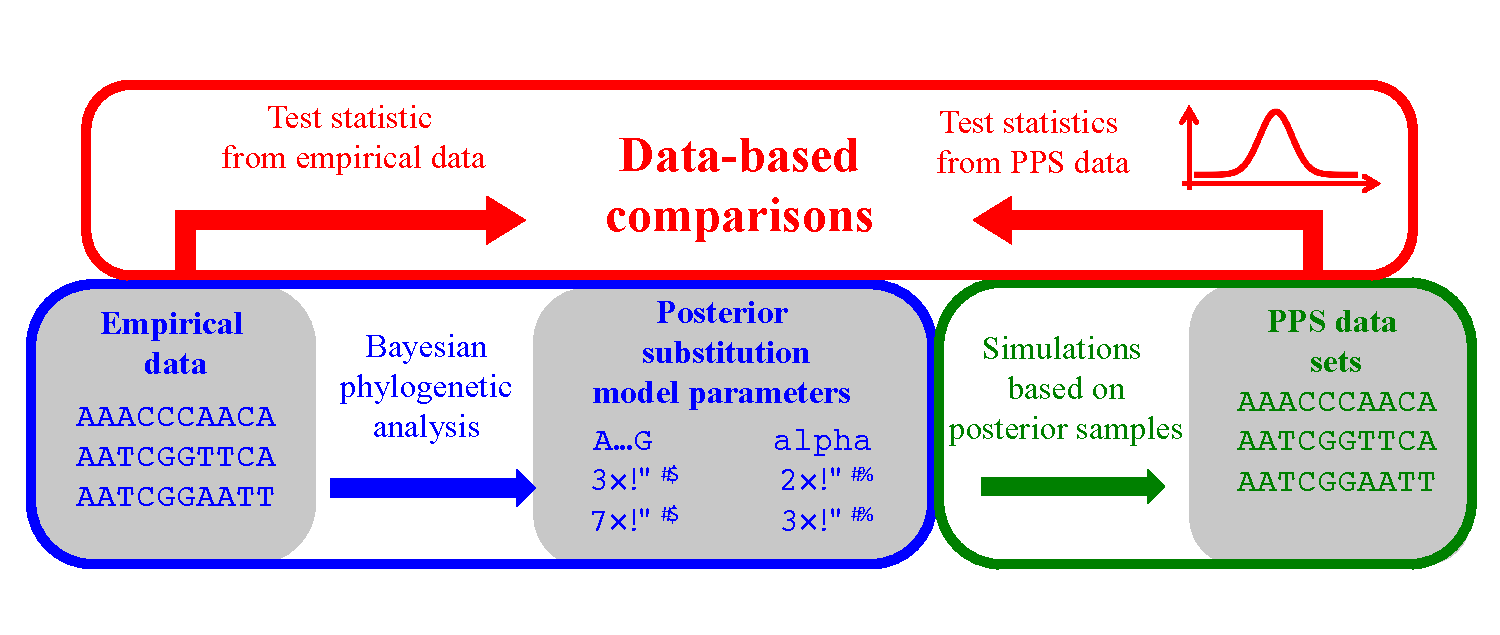
\includegraphics[width=0.8\textwidth]{figures/Adequacy}
  \end{figure}
  Simulated data with estimated parameter should be similar to the empirical data



\end{frame}
